% =============================================================================
% CHAPTER 4 — THE PROPOSED METHOD: PATHCAST
% Thesis: FlowJanus / PATHCAST
% Pipeline: MSR → Event Log → Process Mining → Markov → Monte Carlo (+ ML)
% =============================================================================

\chapter{The Proposed Method: PATHCAST}
\label{ch:method}

This chapter presents the formal specification of the proposed method, 
PATHCAST. The method integrates process mining, 
Markov chain estimation, Monte Carlo simulation, and machine learning into a 
unified pipeline that transforms heterogeneous software repository data into 
probabilistic process forecasts.

Section~\ref{sec:method-overview} provides the architectural overview and 
defines the formal pipeline. Sections~\ref{sec:stage1} 
through~\ref{sec:stage4} formalize each pipeline stage with input/output 
contracts, algorithms, and correctness properties. 
Section~\ref{sec:ml-component} specifies the machine learning enhancement 
component. Section~\ref{sec:integration} formalizes the inter-stage data 
contracts and the end-to-end pipeline composition. 
Section~\ref{sec:method-properties} establishes the formal properties and 
theoretical guarantees of the integrated method. 
Section~\ref{sec:method-summary} synthesizes the contributions.


% =============================================================================
% 4.1 METHOD OVERVIEW
% =============================================================================
\section{Architectural Overview}
\label{sec:method-overview}
These principles ensure that PATHCAST is not just a functional pipeline, but a methodologically sound system with formal properties that guarantee consistency, interpretability, and extensibility.

\subsection{Pipeline Definition}
\label{sec:pipeline-def}

PATHCAST is defined as a composition of four sequential transformation 
stages and one parallel enhancement component:

\begin{definition}[PATHCAST Pipeline]
\label{def:pipeline}
The PATHCAST pipeline is a function composition:
\begin{equation}
\label{eq:pipeline}
\mathcal{F} = \mathcal{S}_4 \circ \mathcal{S}_3 \circ \mathcal{S}_2 \circ \mathcal{S}_1
\end{equation}
where:
\begin{align}
\mathcal{S}_1 &: \mathcal{R} \to \mathcal{L} 
    && \text{(Event Log Construction)} \label{eq:stage1-sig} \\
\mathcal{S}_2 &: \mathcal{L} \to (M, \Phi) 
    && \text{(Process Mining)} \label{eq:stage2-sig} \\
\mathcal{S}_3 &: (\mathcal{L}, M) \to (P, N, B, \hat{F}) 
    && \text{(Markov Estimation)} \label{eq:stage3-sig} \\
\mathcal{S}_4 &: (P, \hat{F}, s_0, M_{\text{sim}}) \to \hat{\mathcal{D}} 
    && \text{(Monte Carlo Simulation)} \label{eq:stage4-sig}
\end{align}
and a parallel component:
\begin{equation}
\mathcal{S}_{\text{ML}} : (\mathcal{L}, \Phi, P, N) \to \hat{f}
    \quad \text{(ML Enhancement)} \label{eq:ml-sig}
\end{equation}
\end{definition}

The notation is defined as follows: $\mathcal{R}$ denotes the set of software 
repositories; $\mathcal{L}$ denotes a structured event log; $M$ denotes a 
discovered process model; $\Phi$ denotes a process metrics vector; $P$ denotes 
a Markov transition matrix; $N$ denotes the fundamental matrix; $B$ denotes 
the absorption probability matrix; $\hat{F}$ denotes the set of empirical 
sojourn time distributions; $\hat{\mathcal{D}}$ denotes the empirical 
forecast distribution; and $\hat{f}$ denotes a trained ML predictor.

\subsection{Pipeline Architecture}
\label{sec:pipeline-arch}

Figure~\ref{fig:pipeline-architecture} illustrates the complete pipeline 
architecture with data flows between stages.

\begin{figure}[htbp]
\centering
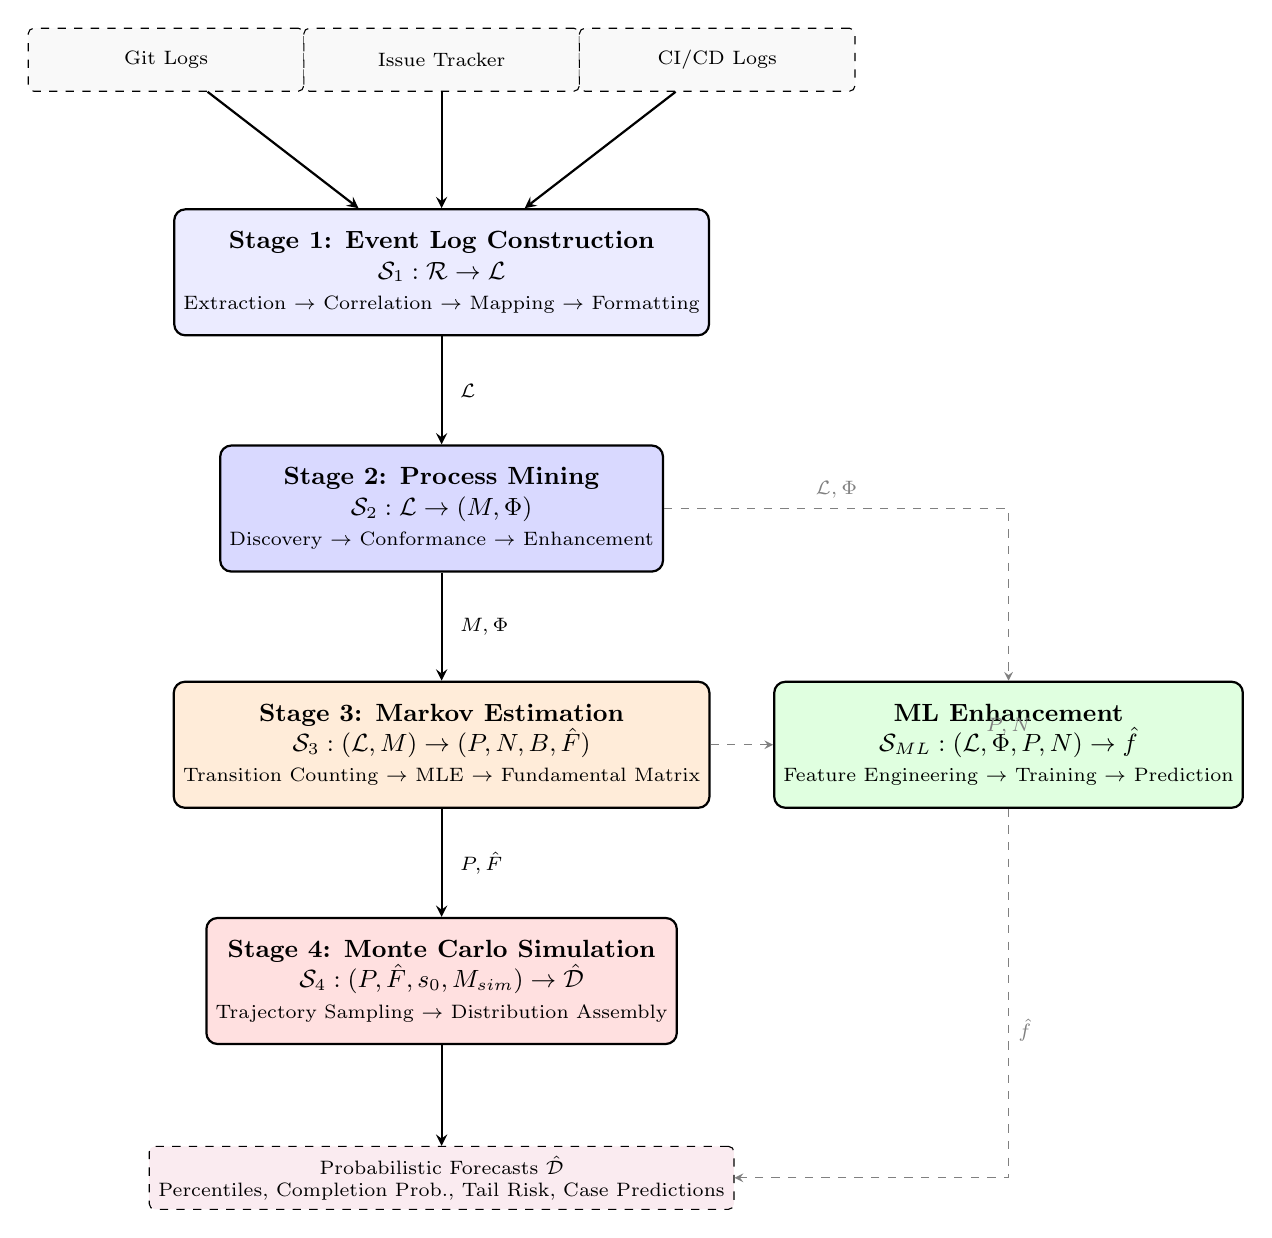
\begin{tikzpicture}[
    node distance=2.2cm,
    stage/.style={rectangle, draw, thick, rounded corners=4pt, 
                  minimum width=5.5cm, minimum height=1.6cm, 
                  align=center, font=\small},
    data/.style={rectangle, draw, dashed, rounded corners=2pt,
                 minimum width=3.5cm, minimum height=0.8cm,
                 align=center, font=\scriptsize, fill=gray!5},
    arrow/.style={->, thick, >=stealth},
    darrow/.style={->, dashed, >=stealth, gray},
    lbl/.style={font=\scriptsize, midway, right, xshift=3pt}
]
    % Sources
    \node[data] (git) at (-3.5, 0) {Git Logs};
    \node[data] (jira) at (0, 0) {Issue Tracker};
    \node[data] (ci) at (3.5, 0) {CI/CD Logs};
    
    % Stage 1
    \node[stage, fill=blue!8, below of=jira, yshift=-0.5cm] (s1) {
        \textbf{Stage 1: Event Log Construction}\\
        $\mathcal{S}_1 : \mathcal{R} \to \mathcal{L}$\\
        {\scriptsize Extraction $\to$ Correlation $\to$ Mapping $\to$ Formatting}
    };
    
    % Stage 2
    \node[stage, fill=blue!15, below of=s1, yshift=-0.8cm] (s2) {
        \textbf{Stage 2: Process Mining}\\
        $\mathcal{S}_2 : \mathcal{L} \to (M, \Phi)$\\
        {\scriptsize Discovery $\to$ Conformance $\to$ Enhancement}
    };
    
    % Stage 3
    \node[stage, fill=orange!15, below of=s2, yshift=-0.8cm] (s3) {
        \textbf{Stage 3: Markov Estimation}\\
        $\mathcal{S}_3 : (\mathcal{L}, M) \to (P, N, B, \hat{F})$\\
        {\scriptsize Transition Counting $\to$ MLE $\to$ Fundamental Matrix}
    };
    
    % Stage 4
    \node[stage, fill=red!12, below of=s3, yshift=-0.8cm] (s4) {
        \textbf{Stage 4: Monte Carlo Simulation}\\
        $\mathcal{S}_4 : (P, \hat{F}, s_0, M_{\text{sim}}) \to \hat{\mathcal{D}}$\\
        {\scriptsize Trajectory Sampling $\to$ Distribution Assembly}
    };
    
    % ML Component
    \node[stage, fill=green!12, right of=s3, xshift=5cm] (ml) {
        \textbf{ML Enhancement}\\
        $\mathcal{S}_{\text{ML}} : (\mathcal{L}, \Phi, P, N) \to \hat{f}$\\
        {\scriptsize Feature Engineering $\to$ Training $\to$ Prediction}
    };
    
    % Output
    \node[data, below of=s4, yshift=-0.3cm, minimum width=5.5cm, fill=purple!8] (output) {
        Probabilistic Forecasts $\hat{\mathcal{D}}$\\
        {\scriptsize Percentiles, Completion Prob., Tail Risk, Case Predictions}
    };
    
    % Arrows
    \draw[arrow] (git) -- (s1);
    \draw[arrow] (jira) -- (s1);
    \draw[arrow] (ci) -- (s1);
    \draw[arrow] (s1) -- (s2) node[lbl] {$\mathcal{L}$};
    \draw[arrow] (s2) -- (s3) node[lbl] {$M, \Phi$};
    \draw[arrow] (s3) -- (s4) node[lbl] {$P, \hat{F}$};
    \draw[arrow] (s4) -- (output);
    
    % ML connections
    \draw[darrow] (s2) -| (ml) node[font=\scriptsize, above, pos=0.25] {$\mathcal{L}, \Phi$};
    \draw[darrow] (s3) -- (ml) node[font=\scriptsize, above] {$P, N$};
    \draw[darrow] (ml) |- (output) node[font=\scriptsize, right, pos=0.3] {$\hat{f}$};
    
\end{tikzpicture}
\caption{PATHCAST pipeline architecture. Solid arrows indicate the 
primary sequential pipeline; dashed arrows indicate ML enhancement data flows.}
\label{fig:pipeline-architecture}
\end{figure}


\subsection{Design Principles}
\label{sec:design-principles}

The pipeline architecture is governed by three design principles:

\textbf{Principle 1 (Empirical Grounding):} Every model parameter is 
estimated from observed data, never assumed \emph{a priori}. The transition 
matrix $P$ is estimated from event log counts; sojourn distributions 
$\hat{F}$ are constructed from observed timestamps; ML features are 
extracted from empirical traces. No distributional assumptions (e.g., 
exponential service times) are imposed unless empirically validated.

\textbf{Principle 2 (Stage Composability):} Each stage has a formally 
defined input/output contract (Definitions~\ref{def:contract-s1} 
through~\ref{def:contract-s4}). Stages can be independently tested, 
replaced, or extended without affecting other stages, provided the 
contract is preserved.

\textbf{Principle 3 (Distributional Outputs):} The pipeline produces 
probability distributions, not point estimates. Every forecast is a 
collection of $M_{\text{sim}}$ simulated outcomes from which percentiles, 
intervals, and tail probabilities are extracted. This design supports 
risk-aware decision-making without requiring downstream consumers to 
understand the internal mechanics of the pipeline.

\subsection{Architectural Overview}
\label{sec:spaf-overview}
\begin{figure}
    \centering
    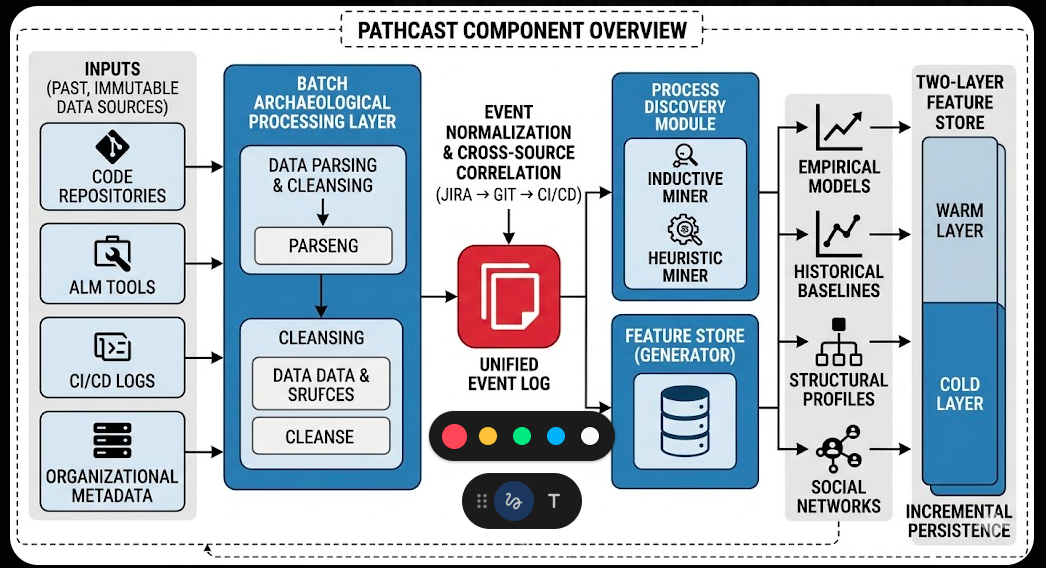
\includegraphics[width=1\linewidth]{figures/path-cast-component-overview.png}
    \caption{Path Cast Overview}
    \label{fig:pathcast-architecture}
\end{figure}
Figure~\ref{fig:pathcast-architecture} presents the architectural overview of
the PATHCAST component, which operates on the temporal dimension of the past.
The framework ingests historical, immutable data sources (code repositories,
ALM tools, CI/CD logs, and organizational metadata) through a batch
archaeological processing layer. The pipeline produces a unified event log
through event normalization and cross-source correlation (Jira $\to$
Git $\to$ CI/CD), which feeds both the process discovery module (Inductive
Miner, Heuristic Miner) and the feature store. The outputs of the PATHCAST
component, empirical models, historical baselines, structural profiles,
and social networks, are persisted incrementally in a two-layer feature
store (cold and warm layers) that serves as the input substrate for the
forecasting stages described in Sections~\ref{sec:stage2}
through~\ref{sec:stage4}.

% =============================================================================
% 4.2 STAGE 1: EVENT LOG CONSTRUCTION (PATHCAST)
% =============================================================================
\section{Stage 1: Event Log Construction}
\label{sec:stage1}

Stage 1 implements the PATHCAST Framework 
component, which transforms heterogeneous software repository data into 
structured event logs suitable for process mining.

\subsection{Formal Specification}
\label{sec:s1-formal}

\begin{definition}[Stage 1 Contract]
\label{def:contract-s1}
\textbf{Input:} A set of software repositories 
$\mathcal{R} = \{r_1, r_2, \ldots, r_n\}$, where each repository $r_i$ 
contains one or more data sources 
$r_i = \{D_i^{(1)}, D_i^{(2)}, \ldots, D_i^{(k_i)}\}$, with each data 
source $D_i^{(j)}$ being a time-ordered sequence of raw events from a 
specific tool (Git, Jira, CI/CD, etc.).

\textbf{Output:} A structured event log 
$\mathcal{L} = \{\sigma_c \mid c \in \mathcal{C}\}$, where $\mathcal{C}$ 
is the set of identified cases and each trace 
$\sigma_c = \langle e_1, e_2, \ldots, e_{|\sigma_c|} \rangle$ is an 
ordered sequence of events satisfying Definition~\ref{def:event-log}.

\textbf{Postconditions:}
\begin{enumerate}
    \item Every event $e \in \sigma_c$ has a valid case identifier, 
    activity name, and timestamp.
    \item Events within each trace are ordered by timestamp: 
    $\tau(e_k) \leq \tau(e_{k+1})$ for all consecutive pairs.
    \item The activity names belong to a defined SDLC activity taxonomy 
    $\mathcal{A}$.
\end{enumerate}
\end{definition}

Stage 1 is decomposed into four sequential sub-operations:

\begin{equation}
\label{eq:s1-decomposition}
\mathcal{S}_1 = \textsc{Format} \circ \textsc{Map} \circ \textsc{Correlate} \circ \textsc{Extract}
\end{equation}


\subsection{Event Extraction}
\label{sec:s1-extraction}

The extraction function parses each data source and produces a set of 
raw events:

\begin{definition}[Raw Event]
\label{def:raw-event}
A raw event is a tuple $e^{\text{raw}} = (ts, src, type, payload)$ where:
\begin{itemize}
    \item $ts \in \mathbb{R}$ is the timestamp;
    \item $src \in \{\texttt{git}, \texttt{jira}, \texttt{ci}, \texttt{review}\}$ 
    identifies the source system;
    \item $type$ is the event type within the source 
    (e.g., \texttt{commit}, \texttt{status\_change}, \texttt{build\_result});
    \item $payload$ is a source-specific attribute map.
\end{itemize}
\end{definition}

Each data source has a dedicated extractor:

\begin{definition}[Source Extractors]
\label{def:extractors}
\begin{align}
\textsc{Extract}_{\text{git}} &: D^{(\text{git})} \to \{e^{\text{raw}}\}
    & \text{parses commit history} \label{eq:extract-git} \\
\textsc{Extract}_{\text{jira}} &: D^{(\text{jira})} \to \{e^{\text{raw}}\}
    & \text{parses issue transitions} \label{eq:extract-jira} \\
\textsc{Extract}_{\text{ci}} &: D^{(\text{ci})} \to \{e^{\text{raw}}\}
    & \text{parses build/deploy events} \label{eq:extract-ci} \\
\textsc{Extract}_{\text{review}} &: D^{(\text{review})} \to \{e^{\text{raw}}\}
    & \text{parses PR lifecycle events} \label{eq:extract-review}
\end{align}
\end{definition}

The union of all extracted events forms the raw event pool:

\begin{equation}
\label{eq:raw-pool}
E^{\text{raw}} = \bigcup_{i=1}^{n} \bigcup_{j=1}^{k_i} 
    \textsc{Extract}_{src(D_i^{(j)})}(D_i^{(j)})
\end{equation}

Table~\ref{tab:event-extraction} specifies the extraction mapping for each 
source type.

\begin{table}[htbp]
\centering
\caption{Event extraction mapping per data source.}
\label{tab:event-extraction}
\small
\begin{tabular}{llll}
\toprule
\textbf{Source} & \textbf{Raw Event Type} & \textbf{Timestamp Source} & \textbf{Key Payload Attributes} \\
\midrule
Git & \texttt{commit} & Author date & hash, author, files, message \\
    & \texttt{merge} & Committer date & source branch, target branch \\
\midrule
Jira & \texttt{status\_change} & Changelog timestamp & from\_status, to\_status, assignee \\
     & \texttt{created} & Creation timestamp & reporter, priority, type \\
     & \texttt{assigned} & Changelog timestamp & from\_assignee, to\_assignee \\
\midrule
CI/CD & \texttt{build\_start} & Build start time & pipeline, trigger, branch \\
      & \texttt{build\_end} & Build end time & result (pass/fail), duration \\
      & \texttt{deploy} & Deploy timestamp & environment, version \\
\midrule
Review & \texttt{pr\_opened} & PR creation time & author, base branch \\
       & \texttt{review\_submitted} & Review timestamp & reviewer, decision \\
       & \texttt{pr\_merged} & Merge timestamp & merge method \\
       & \texttt{pr\_closed} & Close timestamp & reason \\
\bottomrule
\end{tabular}
\end{table}


\subsection{Case Correlation}
\label{sec:s1-correlation}

Case correlation assigns each raw event to a process instance (case). This 
is the most challenging sub-operation in software process mining, because 
events from different tools use different identifiers for the same logical 
unit of work.

\begin{definition}[Case Correlation Function]
\label{def:correlation}
A case correlation function is a mapping:
\begin{equation}
\label{eq:correlation}
\kappa : E^{\text{raw}} \to \mathcal{C} \cup \{\bot\}
\end{equation}
where $\mathcal{C}$ is the set of identified cases and $\bot$ indicates 
an uncorrelated event (which is discarded from the final log).
\end{definition}

The correlation function is implemented as a cascade of strategies, applied 
in order of decreasing specificity:

\begin{algorithm}[htbp]
\caption{Case Correlation Cascade}
\label{alg:correlation}
\begin{algorithmic}[1]
\REQUIRE Raw event pool $E^{\text{raw}}$, correlation configuration $\mathcal{K}$
\ENSURE Case-annotated event set $E^{\text{corr}} \subseteq E^{\text{raw}} \times \mathcal{C}$
\STATE Initialize $E^{\text{corr}} \gets \emptyset$, $E^{\text{pending}} \gets E^{\text{raw}}$
\FOR{each strategy $\kappa_k \in \mathcal{K}$ in priority order}
    \FOR{each event $e \in E^{\text{pending}}$}
        \STATE $c \gets \kappa_k(e)$
        \IF{$c \neq \bot$}
            \STATE $E^{\text{corr}} \gets E^{\text{corr}} \cup \{(e, c)\}$
            \STATE $E^{\text{pending}} \gets E^{\text{pending}} \setminus \{e\}$
        \ENDIF
    \ENDFOR
\ENDFOR
\STATE Report $|E^{\text{pending}}|$ uncorrelated events
\RETURN $E^{\text{corr}}$
\end{algorithmic}
\end{algorithm}

Three correlation strategies are defined:

\textbf{Strategy $\kappa_1$ (Explicit Reference):} Extracts issue keys from 
structured fields. For Jira events, the issue key is the case identifier 
directly. For Git commits, the message is parsed with a configurable regex 
pattern (e.g., \texttt{/([A-Z]+-\textbackslash d+)/}) to extract issue 
references. For CI/CD events, the triggering commit or branch name may 
contain issue references. For pull requests, the linked issue field or 
branch naming convention provides the reference.

Formally:
\begin{equation}
\label{eq:kappa1}
\kappa_1(e) = \begin{cases}
    \text{issue\_key}(e.\text{payload}) & \text{if extractable} \\
    \bot & \text{otherwise}
\end{cases}
\end{equation}

\textbf{Strategy $\kappa_2$ (Structural Link):} Uses platform-provided 
relationships that do not require text parsing. Examples include: GitHub 
pull request $\to$ linked issue associations; CI/CD build $\to$ triggering 
commit $\to$ pull request chains; and Jira sub-task $\to$ parent issue 
hierarchies.

\textbf{Strategy $\kappa_3$ (Heuristic):} For events not resolved by 
$\kappa_1$ or $\kappa_2$, applies heuristic rules based on temporal 
proximity, author identity, and file overlap. For example, a commit by 
author $a$ at time $t$ may be assigned to the active issue of $a$ at $t$ 
if no explicit reference exists.

\begin{definition}[Correlation Quality Metrics]
\label{def:corr-quality}
The quality of case correlation is measured by:
\begin{align}
\text{Coverage} &= \frac{|E^{\text{corr}}|}{|E^{\text{raw}}|} 
    \label{eq:corr-coverage} \\
\text{Ambiguity Rate} &= \frac{|\{e \in E^{\text{raw}} : |\kappa(e)| > 1\}|}{|E^{\text{raw}}|}
    \label{eq:corr-ambiguity}
\end{align}
where $|\kappa(e)| > 1$ indicates an event matching multiple cases. 
Ambiguous events are assigned to the most recent matching case by default, 
or flagged for manual resolution.
\end{definition}


\subsection{Activity Mapping}
\label{sec:s1-mapping}

Activity mapping standardizes heterogeneous event types into a common SDLC 
activity taxonomy.

\begin{definition}[SDLC Activity Taxonomy]
\label{def:activity-taxonomy}
The activity taxonomy is a finite set of canonical SDLC activities:
\begin{equation}
\label{eq:taxonomy}
\mathcal{A} = \{\texttt{created}, \texttt{backlog}, \texttt{in\_progress}, 
    \texttt{review}, \texttt{testing}, \texttt{build}, \texttt{deploy}, 
    \texttt{done}, \texttt{cancelled}\}
\end{equation}
\end{definition}

\begin{definition}[Activity Mapping Function]
\label{def:activity-map}
An activity mapping function $\mu$ transforms raw event types into 
canonical activities:
\begin{equation}
\label{eq:activity-map}
\mu : (src, type, payload) \to \mathcal{A} \cup \{\bot\}
\end{equation}
where $\bot$ indicates an event that does not map to any SDLC activity 
(e.g., a comment added to an issue, which is not a state transition).
\end{definition}

The mapping is implemented as a configurable lookup table. 
Table~\ref{tab:activity-mapping} shows the default mapping for common 
source event types.

\begin{table}[htbp]
\centering
\caption{Default activity mapping from source event types to SDLC taxonomy.}
\label{tab:activity-mapping}
\small
\begin{tabular}{lll}
\toprule
\textbf{Source} & \textbf{Raw Event Type / Condition} & \textbf{Mapped Activity} \\
\midrule
Jira & \texttt{status\_change} $\to$ ``To Do'' & \texttt{backlog} \\
Jira & \texttt{status\_change} $\to$ ``In Progress'' & \texttt{in\_progress} \\
Jira & \texttt{status\_change} $\to$ ``In Review'' & \texttt{review} \\
Jira & \texttt{status\_change} $\to$ ``Done'' & \texttt{done} \\
Git  & \texttt{commit} (first in case) & \texttt{in\_progress} \\
Review & \texttt{pr\_opened} & \texttt{review} \\
Review & \texttt{review\_submitted} (approved) & \texttt{review} \\
CI/CD & \texttt{build\_end} (result=pass) & \texttt{build} \\
CI/CD & \texttt{build\_end} (result=fail) & \texttt{build} \\
CI/CD & \texttt{deploy} & \texttt{deploy} \\
\bottomrule
\end{tabular}
\end{table}


\subsection{Event Log Formatting and Filtering}
\label{sec:s1-formatting}

The final sub-operation assembles correlated, mapped events into a 
structured event log.

\begin{definition}[Structured Event]
\label{def:structured-event}
A structured event is a tuple $e = (\kappa(e), \mu(e), \tau(e), \rho(e), \omega(e))$ where:
\begin{itemize}
    \item $\kappa(e) \in \mathcal{C}$ is the case identifier;
    \item $\mu(e) \in \mathcal{A}$ is the canonical activity;
    \item $\tau(e) \in \mathbb{R}$ is the timestamp;
    \item $\rho(e)$ is the resource (author/assignee);
    \item $\omega(e)$ is an attribute map with source-specific metadata.
\end{itemize}
\end{definition}

Before constructing the final log, two filtering operations are applied:

\textbf{Bot Filtering:} Events attributed to known automated accounts 
(Dependabot, Renovate, CI service accounts) are removed to prevent 
distortion of process models. The bot list is configurable and includes 
both known bots and accounts with commit frequency exceeding a threshold 
$\theta_{\text{bot}}$ (e.g., $> 50$ commits/day).

\textbf{Deduplication:} When multiple raw events map to the same 
$(case, activity, timestamp)$ triple, only the first occurrence is 
retained.

The output event log is:

\begin{equation}
\label{eq:final-log}
\mathcal{L} = \left\{ \sigma_c = \langle e_1, e_2, \ldots, e_{|\sigma_c|} \rangle 
    \;\middle|\; c \in \mathcal{C}, \; 
    \tau(e_k) \leq \tau(e_{k+1}) \; \forall k \right\}
\end{equation}

\subsection{Log Quality Assessment}
\label{sec:s1-quality}

Before proceeding to Stage 2, the event log is assessed for quality:

\begin{definition}[Log Quality Metrics]
\label{def:log-quality}
\begin{align}
\text{Completeness} &= \frac{|\{c \in \mathcal{C} : \sigma_c \text{ reaches an absorbing activity}\}|}{|\mathcal{C}|} 
    \label{eq:log-completeness} \\
\text{Trace Length}(\mathcal{L}) &= \frac{1}{|\mathcal{C}|} \sum_{c \in \mathcal{C}} |\sigma_c|
    \label{eq:trace-length} \\
\text{Activity Coverage} &= \frac{|\{\mu(e) : e \in \mathcal{L}\}|}{|\mathcal{A}|}
    \label{eq:activity-coverage} \\
\text{Variant Count} &= |\{\text{unique activity sequences in } \mathcal{L}\}|
    \label{eq:variant-count}
\end{align}
\end{definition}

Logs with completeness below a threshold $\theta_{\text{comp}}$ (e.g., 0.5) 
or activity coverage below $\theta_{\text{cov}}$ (e.g., 0.6) indicate 
insufficient data for reliable process mining and trigger a warning in the 
pipeline.


% =============================================================================
% 4.3 STAGE 2: PROCESS MINING
% =============================================================================
\section{Stage 2: Process Mining}
\label{sec:stage2}

\subsection{Entropy of Process Variants}
\label{sec:variant-entropy}

Beyond variant count, the diversity of execution paths in a process log
can be quantified through information-theoretic measures. The Shannon
entropy of process variants~\cite{shannon1948mathematical} captures not
only how many distinct paths exist, but how uniformly distributed the
cases are across those paths.

\begin{definition}[Variant Entropy]
\label{def:variant-entropy}
Let $V = \{v_1, v_2, \ldots, v_k\}$ be the set of distinct trace variants
in event log $\mathcal{L}$, and let $p(v_i) = \frac{|\{c \in \mathcal{L}
\mid \sigma_c = v_i\}|}{|\mathcal{L}|}$ be the relative frequency of variant
$v_i$. The variant entropy is defined as:
\begin{equation}
H(V) = -\sum_{v \in V} p(v) \log_2 p(v)
\label{eq:variant-entropy}
\end{equation}
\end{definition}

Variant entropy satisfies $0 \leq H(V) \leq \log_2 |V|$. The lower bound
$H(V) = 0$ occurs when all cases follow a single variant, indicating a
fully deterministic process. The upper bound $H(V) = \log_2 |V|$ is reached
when cases are uniformly distributed across all variants, indicating maximum
behavioral diversity. A normalized variant entropy can be defined as:

\begin{equation}
H_{\text{norm}}(V) = \frac{H(V)}{\log_2 |V|}
\label{eq:variant-entropy-norm}
\end{equation}

\noindent providing a scale-independent measure in $[0, 1]$ that enables
comparison across processes with different numbers of
variants~\cite{aalst2016process}.

In the context of PATHCAST, variant entropy serves as a proxy for
process complexity and predictability. Processes with high $H_{\text{norm}}(V)$
exhibit diverse execution patterns, suggesting weaker structural regularity
and, consequently, greater forecasting difficulty. This metric complements
the discovered process model $M$ by quantifying behavioral dispersion
independently of model structure, and is incorporated as a candidate feature
for the ML component in Stage~4.

\begin{definition}[Stage 2 Contract]
\label{def:contract-s2}
\textbf{Input:} A structured event log $\mathcal{L}$ satisfying the
postconditions of Definition~\ref{def:contract-s1}.

\textbf{Output:} A tuple $(M, \Phi, S)$ where:
\begin{itemize}
    \item $M$ is a discovered process model (process tree or Petri net);
    \item $\Phi = (\phi_{\text{fit}}, \phi_{\text{prec}},
    \phi_{\text{gen}}, \phi_{\text{perf}})$ is a process metrics vector
    containing fitness, precision, generalization, and performance
    metrics;
    \item $S = (S_T, S_A)$ is the SDLC state space partitioned into
    transient states $S_T$ and absorbing states $S_A$.
\end{itemize}

\textbf{Postconditions:}
\begin{enumerate}
    \item $M$ is a sound process model (no deadlocks, no livelocks).
    \item $\phi_{\text{fit}} = \text{fitness}(\mathcal{L}, M) \in [0, 1]$.
    \item $\phi_{\text{prec}} = \text{precision}(\mathcal{L}, M) \in [0, 1]$.
    \item $\phi_{\text{perf}}$ includes per-activity sojourn time
    statistics.
    \item $|S_T| \geq 1$ and $|S_A| \geq 1$.
    \item Every activity $a \in \mathcal{A}$ observed in $\mathcal{L}$ is
    mapped to exactly one state $s \in S_T \cup S_A$.
\end{enumerate}
\end{definition}

\subsection{Process Discovery}
\label{sec:s2-discovery}

The discovery step applies the Inductive Miner algorithm 
(Section~\ref{sec:process-discovery}) to produce a process tree $M$:

\begin{equation}
\label{eq:discovery}
M = \textsc{InductiveMiner}(\mathcal{L}, \theta_{\text{noise}})
\end{equation}

where $\theta_{\text{noise}} \in [0, 1]$ is the noise filtering threshold 
of the Inductive Miner Infrequent (IMf) variant. The threshold controls 
the trade-off between fitness (higher $\theta_{\text{noise}}$ filters more 
infrequent behavior) and generalization (lower $\theta_{\text{noise}}$ 
retains more observed variants).

The Inductive Miner is chosen because it guarantees:

\begin{property}[Soundness Guarantee]
\label{prop:soundness}
The process tree $M$ produced by the Inductive Miner is guaranteed to be 
sound: it has a well-defined initial marking, a well-defined final marking, 
and every reachable marking can reach the final 
marking~\cite{leemans2013discovering}. This property ensures that 
conformance checking (next step) is well-defined.
\end{property}

\begin{property}[Perfect Fitness by Construction]
\label{prop:fitness}
When $\theta_{\text{noise}} = 0$, the Inductive Miner produces a model 
with $\text{fitness}(\mathcal{L}, M) = 1.0$. With noise filtering 
($\theta_{\text{noise}} > 0$), fitness may be less than 1.0, but the 
model remains sound.
\end{property}


\subsection{Conformance Checking}
\label{sec:s2-conformance}

Conformance checking evaluates the relationship between the discovered 
model $M$ and the event log $\mathcal{L}$, producing quality metrics:

\begin{equation}
\label{eq:conformance}
\phi_{\text{fit}} = \text{fitness}(\mathcal{L}, M), \quad 
\phi_{\text{prec}} = \text{precision}(\mathcal{L}, M), \quad
\phi_{\text{gen}} = \text{generalization}(\mathcal{L}, M)
\end{equation}

computed using alignment-based methods 
(Definition~\ref{def:alignment}). These metrics serve dual purposes:

\textbf{Model validation:} If fitness or precision are below acceptable 
thresholds (e.g., $\phi_{\text{fit}} < 0.7$), the discovery step is 
re-executed with adjusted parameters.

\textbf{Case-level conformance features:} For each individual trace 
$\sigma_c$, the alignment cost provides a \emph{conformance score} 
that quantifies how much the case deviates from the typical process. 
This per-case score becomes a feature for the ML component 
(Section~\ref{sec:ml-component}).

\begin{equation}
\label{eq:case-conformance}
\phi_{\text{conf}}(c) = 1 - \frac{\text{cost}(\text{alignment}(\sigma_c, M))}{\text{cost}(\text{worst\_alignment}(\sigma_c, M))}
\end{equation}


\subsection{Performance Enhancement}
\label{sec:s2-enhancement}

Performance enhancement annotates the process model with temporal 
information extracted from the event log:

\begin{definition}[Per-Activity Performance Metrics]
\label{def:performance-metrics}
For each activity $a \in \mathcal{A}$, the following metrics are computed 
from the event log:
\begin{align}
\bar{d}_a &= \frac{1}{|E_a|} \sum_{e \in E_a} d(e) 
    && \text{(mean sojourn time)} \label{eq:mean-sojourn} \\
s_a^2 &= \frac{1}{|E_a| - 1} \sum_{e \in E_a} (d(e) - \bar{d}_a)^2 
    && \text{(sojourn time variance)} \label{eq:var-sojourn} \\
\tilde{d}_a &= \text{median}(\{d(e) : e \in E_a\})
    && \text{(median sojourn time)} \label{eq:median-sojourn}
\end{align}
where $E_a = \{e \in \mathcal{L} : \mu(e) = a\}$ is the set of events 
with activity $a$, and $d(e)$ is the sojourn time (duration between 
event $e$ and the next event in the same trace).
\end{definition}

Additionally, per-transition waiting times are computed:

\begin{equation}
\label{eq:waiting-time}
w_{a \to b} = \frac{1}{|T_{a \to b}|} \sum_{(e_k, e_{k+1}) \in T_{a \to b}} 
    [\tau(e_{k+1}) - \tau(e_k)]
\end{equation}

where $T_{a \to b}$ is the set of consecutive event pairs where 
$\mu(e_k) = a$ and $\mu(e_{k+1}) = b$.

The complete metrics vector is:

\begin{equation}
\label{eq:phi}
\Phi = \left( \phi_{\text{fit}}, \phi_{\text{prec}}, \phi_{\text{gen}}, 
    \{\bar{d}_a, s_a^2, \tilde{d}_a\}_{a \in \mathcal{A}}, 
    \{w_{a \to b}\}_{(a,b) \in \mathcal{A}^2} \right)
\end{equation}


\subsection{State Space Extraction}
\label{sec:s2-states}

The final operation of Stage 2 extracts the state space for Markov modeling:

\begin{definition}[SDLC State Space]
\label{def:state-space}
From the discovered model $M$ and the event log $\mathcal{L}$, the SDLC 
state space is defined as:
\begin{equation}
\label{eq:state-space}
S = S_T \cup S_A
\end{equation}
where $S_T$ is the set of transient states (activities observed in 
non-terminal positions of traces) and $S_A$ is the set of absorbing 
states (terminal activities: \texttt{done}, \texttt{cancelled}).

The state space satisfies $|S_T| \geq 1$ and $|S_A| \geq 1$.
\end{definition}

The state space $S$, together with the event log $\mathcal{L}$ and 
model $M$, is passed to Stage 3 for Markov estimation.
% =============================================================================
% CHAPTER 4 — PART 2: STAGES 3-4, ML, INTEGRATION, PROPERTIES
% Continues from chapter4_part1.tex
% =============================================================================


% =============================================================================
% 4.4 STAGE 3: MARKOV ESTIMATION
% =============================================================================
\section{Stage 3: Stochastic Modeling}
\label{sec:stage3}
These metrics constitute the empirical basis for constructing the residence time distributions used in Stage 3, enabling the transition from a structural model to a temporal stochastic model.

Although aggregated metrics (mean, variance, median) are used in the descriptive analysis, PATHCAST uses the full empirical distribution of residence times for sampling in Stage 4.

\begin{remark}[Empirical Distributions]
\label{rem:empirical-distributions}
Although aggregate metrics (mean, variance, median) are used in descriptive
analysis, PATHCAST employs the complete empirical distribution of
sojourn times for sampling in Stage~4. This choice preserves the
distributional shape, including skewness and heavy tails commonly observed
in software development lead
times~\cite{little2011factory, flyvbjerg2022empirical}, avoiding the
information loss inherent in parametric assumptions. Software development
lead times and project outcomes exhibit heavy-tailed distributions where
the variance may be undefined~\cite{flyvbjerg2022empirical}, rendering
mean-based parametric models inadequate for capturing the true risk
profile of process durations. Furthermore, the reproducibility of
empirical findings in software engineering depends on preserving the
original distributional characteristics of the data retrieved from
development repositories~\cite{gonzalezbarahona2014reproducibility}.
Imposing distributional assumptions introduces a methodological confound
that compromises both the validity of individual forecasts and the
reproducibility of the overall pipeline. By sampling directly from
empirical distributions, the Monte Carlo simulation in Stage~4 propagates
the full uncertainty structure of the observed process, preserving
skewness, kurtosis, and heavy tails rather than relying on distributional
fits that may misrepresent tail behavior.
\end{remark}

\subsection{Formal Specification}
\label{sec:s3-formal}

\begin{definition}[Stage 3 Contract]
\label{def:contract-s3}
\textbf{Input:} A structured event log $\mathcal{L}$ and the SDLC state 
space $S = S_T \cup S_A$ extracted by Stage 2 
(Definition~\ref{def:state-space}).

\textbf{Output:} A tuple $(P, N, B, \hat{F}, \pi)$ where:
\begin{itemize}
    \item $P \in \mathbb{R}^{|S| \times |S|}$ is the estimated transition matrix;
    \item $N = (I - Q)^{-1} \in \mathbb{R}^{|S_T| \times |S_T|}$ is the 
    fundamental matrix (Definition~\ref{def:fundamental-matrix});
    \item $B = NR \in \mathbb{R}^{|S_T| \times |S_A|}$ is the absorption 
    probability matrix;
    \item $\hat{F} = \{\hat{F}_s\}_{s \in S_T}$ is the set of empirical 
    sojourn time distributions, one per transient state;
    \item $\pi \in \mathbb{R}^{|S|}$ is the stationary distribution 
    (when defined).
\end{itemize}

\textbf{Preconditions:}
\begin{enumerate}
    \item $|S_T| \geq 1$ and $|S_A| \geq 1$.
    \item Every transient state $s \in S_T$ has at least one observed 
    outgoing transition in $\mathcal{L}$.
\end{enumerate}

\textbf{Postconditions:}
\begin{enumerate}
    \item $P$ is row-stochastic: $P_{ij} \geq 0$ and 
    $\sum_j P_{ij} = 1$ for all $i$.
    \item $(I - Q)$ is invertible (guaranteed by the absorbing property).
    \item $N_{ij} \geq 0$ for all $i, j$ and 
    $\sum_j B_{ij} = 1$ for all $i \in S_T$.
    \item Each $\hat{F}_s$ contains at least $n_{\min}$ observations.
\end{enumerate}
\end{definition}

Stage 3 is decomposed into five operations:

\begin{equation}
\label{eq:s3-decomposition}
\mathcal{S}_3 = \textsc{Stationary} \circ \textsc{Sojourn} \circ 
    \textsc{Absorb} \circ \textsc{Estimate} \circ \textsc{Count}
\end{equation}


\subsection{Transition Counting}
\label{sec:s3-counting}

The first operation iterates over all traces in $\mathcal{L}$, extracting
consecutive state pairs and accumulating counts in a transition count
matrix. The count matrix $C$ constitutes the empirical basis for
estimating transition probabilities, representing the observed frequency
of process dynamics. The initial state distribution $c_0$ provides the
empirical entry point distribution for Monte Carlo simulation.

\begin{property}[Count Consistency]
\label{prop:count-consistency}
For each state $i$, the row sum of the count matrix equals the total
number of transitions originating from state $i$:
\begin{equation}
\sum_{j} C_{ij} = c_{i \cdot}
\label{eq:count-consistency}
\end{equation}
where $c_{i \cdot}$ denotes the total number of observed transitions
departing from state $i$. This property ensures that no transitions are
lost or duplicated during the counting procedure, preserving the
statistical sufficiency of $C$ for maximum likelihood estimation of the
transition probabilities.
\end{property}

The count matrix $C$ is the sufficient statistic for MLE of the transition
probabilities, and its row sums determine the denominator of the
per-state normalization applied in the subsequent estimation step.

\begin{algorithm}[htbp]
\caption{Transition Count Extraction}
\label{alg:counting}
\begin{algorithmic}[1]
\REQUIRE Event log $\mathcal{L}$, state space $S$
\ENSURE Transition count matrix $C \in \mathbb{N}^{|S| \times |S|}$, 
    initial state counts $c_0 \in \mathbb{N}^{|S|}$
\STATE Initialize $C \gets \mathbf{0}^{|S| \times |S|}$, 
    $c_0 \gets \mathbf{0}^{|S|}$
\FOR{each trace $\sigma_c = \langle e_1, \ldots, e_{|\sigma_c|} \rangle \in \mathcal{L}$}
    \STATE $c_0[\mu(e_1)] \gets c_0[\mu(e_1)] + 1$
    \FOR{$k = 1$ to $|\sigma_c| - 1$}
        \STATE $i \gets \mu(e_k)$, \quad $j \gets \mu(e_{k+1})$
        \STATE $C[i][j] \gets C[i][j] + 1$
    \ENDFOR
\ENDFOR
\RETURN $C$, $c_0$
\end{algorithmic}
\end{algorithm}


\subsection{Maximum Likelihood Estimation}
\label{sec:s3-mle}

The transition probabilities are estimated by MLE with optional Laplace 
smoothing:

\begin{equation}
\label{eq:mle-full}
\hat{P}_{ij} = \frac{C_{ij} + \alpha}{\sum_{j'=1}^{|S|} C_{ij'} + \alpha |S|}
\end{equation}

where $\alpha \geq 0$ is the smoothing parameter. When $\alpha = 0$, 
this reduces to the standard MLE $\hat{P}_{ij} = C_{ij} / C_{i \cdot}$ 
(Equation~\ref{eq:mle-transition}).

\begin{property}[MLE Consistency]
\label{prop:mle-consistency}
For $\alpha = 0$, the MLE estimator $\hat{P}$ converges almost surely to 
the true transition matrix $P^*$ as the number of observed traces 
$|\mathcal{L}| \to \infty$, provided every state is visited infinitely 
often~\cite{Spedicato2017}.
\end{property}

Smoothing ($\alpha > 0$) is applied when any row of $C$ contains states 
with zero observed transitions but non-zero transitions are structurally 
plausible. The default value is $\alpha = 1$ (Laplace prior), which 
assigns minimal probability mass to unobserved but possible transitions. 
The choice of $\alpha$ is validated empirically through sensitivity 
analysis in Chapter~\ref{ch:evaluation}.


\subsection{Confidence Assessment of Transition Estimates}
\label{sec:s3-confidence}

Because individual transition probabilities are estimated from finite 
samples, the pipeline computes confidence intervals for each estimate 
to quantify estimation uncertainty.

For a multinomial row with $n_i = C_{i \cdot}$ observations, the 
standard error of $\hat{P}_{ij}$ is:

\begin{equation}
\label{eq:se-transition}
\text{SE}(\hat{P}_{ij}) = \sqrt{\frac{\hat{P}_{ij}(1 - \hat{P}_{ij})}{n_i}}
\end{equation}

An approximate $(1 - \delta)$ confidence interval is:

\begin{equation}
\label{eq:ci-transition}
\hat{P}_{ij} \pm z_{\delta/2} \cdot \text{SE}(\hat{P}_{ij})
\end{equation}

where $z_{\delta/2}$ is the standard normal quantile. Rows with 
$n_i < n_{\min}$ (default $n_{\min} = 30$) are flagged as low-confidence 
estimates, and the pipeline reports a \textbf{confidence grade} for the 
overall transition matrix:

\begin{equation}
\label{eq:confidence-grade}
\text{Grade}(P) = \frac{|\{i \in S_T : n_i \geq n_{\min}\}|}{|S_T|}
\end{equation}

A grade below $\theta_{\text{grade}} = 0.8$ indicates that the event log 
contains insufficient transition data for reliable Markov modeling, and 
the pipeline reports this as a validity caveat.


\subsection{Absorbing Chain Decomposition}
\label{sec:s3-absorbing}
This formulation provides an analytical estimator of the completion time, which serves as a baseline for validating the results obtained through Monte Carlo simulations in Stage 4.

Given the estimated matrix $\hat{P}$, the states are reordered so that 
transient states (elements of $S_T$) precede absorbing states (elements 
of $S_A$):

\begin{equation}
\label{eq:absorbing-decomposition}
\hat{P} = \begin{pmatrix} Q & R \\ \mathbf{0} & I \end{pmatrix}
\end{equation}

where $Q \in \mathbb{R}^{|S_T| \times |S_T|}$ captures transient-to-transient 
dynamics and $R \in \mathbb{R}^{|S_T| \times |S_A|}$ captures 
transient-to-absorbing transitions.

The fundamental matrix and absorption probabilities are computed as:

\begin{align}
N &= (I - Q)^{-1} \label{eq:fundamental-computation} \\
t &= N \cdot \mathbf{1} && \text{(expected steps to absorption)} \label{eq:expected-steps} \\
B &= N \cdot R && \text{(absorption probabilities)} \label{eq:absorption-prob}
\end{align}

\begin{property}[Invertibility]
\label{prop:invertibility}
The matrix $(I - Q)$ is invertible if and only if every transient state 
can eventually reach an absorbing state. This is guaranteed by the 
precondition that $|S_A| \geq 1$ and the structural connectivity of SDLC 
workflows (every work item can eventually be completed or cancelled). If 
the precondition is violated (e.g., a cyclic subgraph with no exit), the 
pipeline detects the singularity and reports a structural error.
\end{property}

\begin{property}[Absorption Certainty]
\label{prop:absorption-certainty}
For an absorbing chain, absorption is certain: starting from any transient 
state, the process reaches an absorbing state with probability 1. Formally, 
$\sum_{a \in S_A} B_{ia} = 1$ for all $i \in S_T$.
\end{property}

The vector $t$ provides the core analytical forecast: $t_i$ is the expected 
number of state transitions from transient state $i$ until absorption. 
Combined with sojourn time distributions, this yields the expected 
lead time in calendar time:

\begin{equation}
\label{eq:expected-lead-time}
\mathbb{E}[\text{LeadTime} \mid s_0 = i] = \sum_{j \in S_T} N_{ij} \cdot \bar{d}_j
\end{equation}

where $\bar{d}_j$ is the mean sojourn time in state $j$ 
(Equation~\ref{eq:mean-sojourn}).


\subsection{Empirical Sojourn Time Distribution Estimation}
\label{sec:s3-sojourn}

For each transient state $s \in S_T$, the empirical sojourn time 
distribution is constructed from observed timestamps:

\begin{definition}[Empirical Sojourn Time Distribution]
\label{def:sojourn-distribution}
For state $s \in S_T$, define the set of observed sojourn times:
\begin{equation}
\label{eq:sojourn-obs}
\mathcal{T}_s = \left\{ \tau(e_{k+1}) - \tau(e_k) \;\middle|\; 
    \mu(e_k) = s, \; (e_k, e_{k+1}) \text{ consecutive in some } \sigma_c \right\}
\end{equation}

The empirical cumulative distribution function is:
\begin{equation}
\label{eq:ecdf}
\hat{F}_s(t) = \frac{1}{|\mathcal{T}_s|} \sum_{\tau \in \mathcal{T}_s} 
    \mathbf{1}[\tau \leq t]
\end{equation}
\end{definition}

The sojourn distributions are stored as sorted arrays of observed values. 
Monte Carlo simulation (Stage 4) samples from these distributions using 
empirical resampling (drawing uniformly from $\mathcal{T}_s$), which 
imposes no parametric assumptions on the shape of sojourn time 
distributions.

\begin{remark}[Non-Parametric Design Choice]
\label{rem:nonparametric}
The decision to use empirical distributions rather than fitted parametric 
distributions (e.g., exponential, log-normal, Weibull) follows Design 
Principle 1 (Empirical Grounding). Software process sojourn times 
frequently exhibit multi-modal, heavy-tailed, or zero-inflated patterns that are poorly captured by standard parametric 
families~\cite{vacanti2015}. Empirical resampling preserves 
these characteristics without requiring distributional assumptions.
\end{remark}


\subsection{Stationary Distribution and WIP Analysis}
\label{sec:s3-stationary}

For the transient subchain $Q$, the stationary distribution is not 
defined (absorption is certain). However, the \emph{quasi-stationary 
distribution} describes the long-run proportion of time spent in each 
transient state, conditional on not yet being absorbed:

\begin{equation}
\label{eq:quasi-stationary}
\tilde{\pi}_j = \frac{\sum_{i \in S_T} \pi_0(i) \cdot N_{ij}}
    {\sum_{i \in S_T} \pi_0(i) \cdot t_i}
\end{equation}

where $\pi_0$ is the initial state distribution estimated from $c_0$ 
(Algorithm~\ref{alg:counting}).

The quasi-stationary distribution provides an interpretable decomposition 
of WIP: $\tilde{\pi}_j$ approximates the fraction of active work items 
expected in state $j$ at any given time. States with disproportionately 
high $\tilde{\pi}_j$ relative to their processing capacity indicate 
bottleneck accumulation.


\subsection{Rework Analysis}
\label{sec:s3-rework}
Rework analysis provides a quantitative breakdown of process inefficiencies, allowing you to identify not only the presence of loops, but also their expected intensity and their impact on lead time.

The simulation algorithm operationalizes the stochastic process defined in Stage 3, producing distributional forecasts that capture both the structural dynamics of the process and its temporal variability, enabling risk-oriented decisions beyond point estimates

A distinctive feature of SDLC processes is the prevalence of rework loops 
(regressive transitions). The Markov model quantifies rework through 
the off-diagonal elements of $N$:

\begin{definition}[Rework Intensity]
\label{def:rework}
The expected number of rework cycles for transition $a \to b$ (where 
$b$ precedes $a$ in the nominal process order) starting from state $i$ 
is:
\begin{equation}
\label{eq:rework-intensity}
R_{i,a \to b} = N_{ia} \cdot P_{ab}
\end{equation}

The total expected rework for a case starting in state $i$ is:
\begin{equation}
\label{eq:total-rework}
R_i^{\text{total}} = \sum_{(a,b) \in \mathcal{E}_{\text{rework}}} R_{i,a \to b}
\end{equation}
where $\mathcal{E}_{\text{rework}} = \{(a, b) \in S_T \times S_T : 
\text{order}(b) < \text{order}(a)\}$ is the set of regressive transitions 
relative to the nominal SDLC ordering.
\end{definition}

For example, if the nominal order is Backlog $\to$ In Progress $\to$ 
Review $\to$ Testing $\to$ Done, then Review $\to$ In Progress is a 
rework transition, and $R_{i, \text{Review} \to \text{InProgress}}$ gives 
the expected number of times a case starting in state $i$ undergoes this 
specific rework cycle.


\subsection{Numerical Example}
\label{sec:s3-example}

To illustrate the computations, consider a simplified SDLC with states 
$S = \{B, P, R, T, D, X\}$ (Backlog, In Progress, Review, Testing, Done, 
Cancelled), where $D$ and $X$ are absorbing. Suppose the event log yields 
the following transition count matrix:

\begin{equation}
\label{eq:example-counts}
C = \bordermatrix{
    & B & P & R & T & D & X \cr
  B & 0 & 85 & 0 & 0 & 5 & 10 \cr
  P & 0 & 0 & 80 & 5 & 0 & 15 \cr
  R & 0 & 25 & 0 & 70 & 0 & 5 \cr
  T & 0 & 10 & 15 & 0 & 70 & 5 \cr
  D & 0 & 0 & 0 & 0 & 0 & 0 \cr
  X & 0 & 0 & 0 & 0 & 0 & 0 \cr
}
\end{equation}

MLE estimation (Equation~\ref{eq:mle-full} with $\alpha = 0$) produces:

\begin{equation}
\label{eq:example-P}
\hat{P} = \begin{pmatrix}
0    & 0.85 & 0    & 0    & 0.05 & 0.10 \\
0    & 0    & 0.80 & 0.05 & 0    & 0.15 \\
0    & 0.25 & 0    & 0.70 & 0    & 0.05 \\
0    & 0.10 & 0.15 & 0    & 0.70 & 0.05 \\
0    & 0    & 0    & 0    & 1    & 0    \\
0    & 0    & 0    & 0    & 0    & 1    \\
\end{pmatrix}
\end{equation}

Extracting the transient submatrix $Q$ and the absorption submatrix $R$:

\begin{equation}
\label{eq:example-QR}
Q = \begin{pmatrix}
0    & 0.85 & 0    & 0    \\
0    & 0    & 0.80 & 0.05 \\
0    & 0.25 & 0    & 0.70 \\
0    & 0.10 & 0.15 & 0    \\
\end{pmatrix}, \quad
R = \begin{pmatrix}
0.05 & 0.10 \\
0    & 0.15 \\
0    & 0.05 \\
0.70 & 0.05 \\
\end{pmatrix}
\end{equation}

Computing the fundamental matrix $N = (I - Q)^{-1}$:

\begin{equation}
\label{eq:example-N}
N = \begin{pmatrix}
1.000 & 1.431 & 1.458 & 1.134 \\
0     & 1.684 & 1.715 & 1.334 \\
0     & 0.675 & 1.688 & 1.054 \\
0     & 0.285 & 0.441 & 1.267 \\
\end{pmatrix}
\end{equation}

The expected steps to absorption (from each transient state):

\begin{equation}
\label{eq:example-t}
t = N \cdot \mathbf{1} = \begin{pmatrix}
5.023 \\ 4.733 \\ 3.417 \\ 1.993
\end{pmatrix}
\end{equation}

\textbf{Interpretation:} A work item starting in Backlog ($B$) visits an 
expected 5.02 states before reaching Done or Cancelled. Starting from 
Testing ($T$), only 1.99 transitions are expected.

The absorption probability matrix:

\begin{equation}
\label{eq:example-B}
B = N \cdot R = \begin{pmatrix}
0.844 & 0.156 \\
0.990 & 0.010 \\
... & ... \\
... & ...
\end{pmatrix}
\end{equation}

\textbf{Note:} The exact values of $N$ and $B$ depend on the numerical 
inversion. The values above are rounded for illustration; the 
implementation uses double-precision floating-point arithmetic. 
Complete numerical validation is provided in Chapter~\ref{ch:evaluation}.

Suppose the mean sojourn times (in hours) are $\bar{d}_B = 48$, 
$\bar{d}_P = 24$, $\bar{d}_R = 8$, $\bar{d}_T = 4$. Then the expected 
lead time from Backlog is:

\begin{equation}
\label{eq:example-lead-time}
\mathbb{E}[\text{LeadTime} \mid s_0 = B] = 
    1.000 \times 48 + 1.431 \times 24 + 1.458 \times 8 + 1.134 \times 4 
    \approx 98.9 \text{ hours}
\end{equation}

This analytical estimate provides a rapid baseline forecast. Stage 4 
refines it by producing the full probability distribution rather than 
a single expected value.


% =============================================================================
% 4.5 STAGE 4: MONTE CARLO SIMULATION
% =============================================================================
\section{Stage 4: Monte Carlo Simulation}
\label{sec:stage4}

Stage 4 generates probabilistic process forecasts by simulating stochastic 
trajectories through the Markov model, sampling state transitions and 
sojourn times from the empirical distributions estimated in Stage 3.

\subsection{Formal Specification}
\label{sec:s4-formal}

\begin{definition}[Stage 4 Contract]
\label{def:contract-s4}
\textbf{Input:} Transition matrix $P$, empirical sojourn distributions 
$\hat{F} = \{\hat{F}_s\}_{s \in S_T}$, initial state $s_0 \in S_T$ 
(or initial distribution $\pi_0$ over $S$), and number of simulations 
$M_{\text{sim}} \in \mathbb{N}$.

\textbf{Output:} An empirical forecast distribution:
\begin{equation}
\label{eq:forecast-distribution}
\hat{\mathcal{D}} = \left\{ \left( T^{(m)}, o^{(m)}, \psi^{(m)} \right) 
    \right\}_{m=1}^{M_{\text{sim}}}
\end{equation}
where for each simulation $m$:
\begin{itemize}
    \item $T^{(m)} \in \mathbb{R}_+$ is the total lead time (sum of 
    sojourn times along the trajectory);
    \item $o^{(m)} \in S_A$ is the terminal (absorbing) state reached;
    \item $\psi^{(m)} = \langle s_0^{(m)}, s_1^{(m)}, \ldots, 
    s_{K^{(m)}}^{(m)} \rangle$ is the state path (trajectory).
\end{itemize}

\textbf{Postconditions:}
\begin{enumerate}
    \item $|\hat{\mathcal{D}}| = M_{\text{sim}}$.
    \item Every trajectory terminates in an absorbing state: 
    $s_{K^{(m)}}^{(m)} \in S_A$ for all $m$.
    \item $T^{(m)} > 0$ for all $m$.
\end{enumerate}
\end{definition}


\subsection{Simulation Algorithm}
\label{sec:s4-algorithm}

The core simulation algorithm generates individual stochastic trajectories:

\begin{algorithm}[htbp]
\caption{Process-Aware Monte Carlo Simulation (Full Specification)}
\label{alg:mc-full}
\begin{algorithmic}[1]
\REQUIRE $P$, $\hat{F}$, $\pi_0$ (or fixed $s_0$), $M_{\text{sim}}$, 
    max steps $K_{\max}$
\ENSURE $\hat{\mathcal{D}} = \{(T^{(m)}, o^{(m)}, \psi^{(m)})\}_{m=1}^{M_{\text{sim}}}$
\STATE $\hat{\mathcal{D}} \gets \emptyset$
\FOR{$m = 1$ to $M_{\text{sim}}$}
    \IF{$s_0$ is fixed}
        \STATE $s \gets s_0$
    \ELSE
        \STATE $s \gets \text{sample from } \pi_0$ 
        \Comment{Weighted random choice}
    \ENDIF
    \STATE $T \gets 0$; $\psi \gets [s]$; $k \gets 0$
    \WHILE{$s \notin S_A$ and $k < K_{\max}$}
        \STATE \textbf{// Sample sojourn time}
        \STATE $\Delta t \gets \text{sample from } \hat{F}_s$ 
        \Comment{Uniform draw from $\mathcal{T}_s$}
        \STATE $T \gets T + \Delta t$
        \STATE \textbf{// Sample next state}
        \STATE $s' \gets \text{categorical}(P[s, :])$
        \Comment{Weighted random choice from row $s$ of $P$}
        \STATE $s \gets s'$; append $s$ to $\psi$; $k \gets k + 1$
    \ENDWHILE
    \IF{$s \notin S_A$}
        \STATE Mark simulation $m$ as \texttt{non-absorbed} 
        \Comment{Safety: exceeded $K_{\max}$}
    \ENDIF
    \STATE $\hat{\mathcal{D}} \gets \hat{\mathcal{D}} \cup 
        \{(T, s, \psi)\}$
\ENDFOR
\RETURN $\hat{\mathcal{D}}$
\end{algorithmic}
\end{algorithm}

The safety parameter $K_{\max}$ prevents infinite loops in degenerate 
cases. For well-formed absorbing chains, the probability of exceeding 
$K_{\max}$ steps decreases exponentially with $K_{\max}$. The default 
value $K_{\max} = 1000$ is conservative; simulations exceeding this 
limit are excluded from forecast aggregation and reported as anomalies.


\subsection{Forecast Extraction}
\label{sec:s4-forecasts}

The forecasts derived from the empirical distribution capture not only the central tendency of the process, but also its variability, uncertainty, and structural execution patterns, enabling informed, risk-oriented decision-making in software development management.

The comparison between the composition of WIP estimated by simulation and the analytical quasi-stationary distribution provides a model cross-validation mechanism, allowing one to assess the consistency between the mathematical formulation and the observed stochastic behavior.


From the empirical distribution $\hat{\mathcal{D}}$, the following 
forecasts are extracted:

\subsubsection{Percentile Lead Time Forecasts}

\begin{definition}[Percentile Forecast]
\label{def:percentile-forecast}
The $\alpha$-percentile lead time forecast is:
\begin{equation}
\label{eq:percentile}
\hat{Q}_\alpha = \inf \left\{ t : \hat{F}_T(t) \geq \alpha \right\}
\end{equation}
where $\hat{F}_T(t) = \frac{1}{M_{\text{sim}}} 
    \sum_{m=1}^{M_{\text{sim}}} \mathbf{1}[T^{(m)} \leq t]$ 
is the empirical CDF of simulated lead times.
\end{definition}

Standard reporting percentiles are P50 (median forecast), P85 (high 
confidence commitment), and P95 (conservative commitment), consistent 
with agile forecasting practice~\cite{vacanti2015}.

\subsubsection{Completion Probability}

\begin{equation}
\label{eq:completion-prob}
\hat{P}(\text{Done}) = \frac{|\{m : o^{(m)} = \texttt{done}\}|}{M_{\text{sim}}}
\end{equation}

This estimates the probability that a work item starting in state $s_0$ 
will eventually reach Done rather than Cancelled.

\subsubsection{Tail Risk}

\begin{definition}[Tail Risk]
\label{def:tail-risk}
For a deadline threshold $\tau_{\text{deadline}}$:
\begin{equation}
\label{eq:tail-risk}
\hat{P}(\text{late}) = \frac{|\{m : T^{(m)} > \tau_{\text{deadline}}\}|}{M_{\text{sim}}}
\end{equation}
\end{definition}

\subsubsection{Path Distribution}

From the collected trajectories $\{\psi^{(m)}\}$, the most frequent 
state paths are identified:

\begin{equation}
\label{eq:path-freq}
\text{freq}(\psi) = \frac{|\{m : \psi^{(m)} = \psi\}|}{M_{\text{sim}}}
\end{equation}

The top-$k$ most frequent paths reveal the dominant process execution 
patterns and the relative prevalence of rework-laden versus direct 
paths.

\subsubsection{WIP Composition}

\begin{equation}
\label{eq:wip-composition}
\hat{\pi}_j^{\text{MC}} = \frac{\sum_{m=1}^{M_{\text{sim}}} 
    \text{time in state } j \text{ during } \psi^{(m)}}
    {\sum_{m=1}^{M_{\text{sim}}} T^{(m)}}
\end{equation}

This provides a simulation-based estimate of WIP composition that can 
be compared with the analytical quasi-stationary distribution 
(Equation~\ref{eq:quasi-stationary}) as a cross-validation.


\subsection{Convergence and Simulation Budget}
\label{sec:s4-convergence}

The accuracy of Monte Carlo estimates depends on $M_{\text{sim}}$. The 
pipeline determines the simulation budget adaptively.

\begin{definition}[Convergence Criterion]
\label{def:convergence}
The simulation is considered converged when the relative half-width of 
the 95\% confidence interval for the median lead time falls below a 
tolerance $\epsilon$:
\begin{equation}
\label{eq:convergence-criterion}
\frac{z_{0.025} \cdot \hat{\sigma}_T / \sqrt{M_{\text{sim}}}}{\hat{Q}_{0.5}} 
    < \epsilon
\end{equation}
where $\hat{\sigma}_T$ is the sample standard deviation of 
$\{T^{(m)}\}$ and $\hat{Q}_{0.5}$ is the current median estimate.
\end{definition}

The default tolerance is $\epsilon = 0.02$ (2\% relative precision). 
The simulation starts with $M_{\text{sim}} = 1{,}000$ and doubles until 
convergence, with a ceiling of $M_{\text{sim}} = 100{,}000$.

\begin{property}[Convergence Rate]
\label{prop:convergence-rate}
The Monte Carlo estimation error for the mean lead time decreases as 
$O(1 / \sqrt{M_{\text{sim}}})$, independent of the number of states 
$|S|$ or the complexity of the sojourn 
distributions~\cite{robert2004monte}. This guarantees that sufficient 
accuracy is achievable for any SDLC process complexity given adequate 
simulation budget.
\end{property}


\subsection{Comparison with Throughput-Based Monte Carlo}
\label{sec:s4-comparison}

While throughput-based approaches treat the process as a black box, the proposed approach explicitly incorporates its structure, enabling interpretable and actionable predictions.


The proposed simulation differs from the throughput-based approach 
of Vacanti~\cite{vacanti2015} in three respects:

\begin{table}[htbp]
\centering
\caption{Comparison between throughput-based and process-aware Monte Carlo.}
\label{tab:mc-comparison}
\begin{tabular}{lll}
\toprule
\textbf{Dimension} & \textbf{Throughput-Based} & \textbf{Process-Aware (Proposed)} \\
\midrule
Process model & None (black box) & PM-discovered (explicit states) \\
Sampling unit & Daily throughput & State transition + sojourn time \\
Rework modeling & Not captured & Explicit via $P_{ab}$ for regressive $(a,b)$ \\
State-specific delays & Not captured & Per-state $\hat{F}_s$ \\
Path information & Not available & Full trajectory $\psi^{(m)}$ \\
Distributional & Completion date only & Lead time + outcome + path + WIP \\
\quad outputs & & \\
\bottomrule
\end{tabular}
\end{table}

The process-aware approach produces richer information at the cost of 
requiring a structured event log (Stage 1) and a Markov model (Stage 3), 
which the throughput-based approach does not need.


% =============================================================================
% 4.6 ML ENHANCEMENT COMPONENT
% =============================================================================
\section{Machine Learning Enhancement Component}
\label{sec:ml-component}

The ML component operates in parallel with the primary pipeline, using 
features derived from process mining and Markov analysis to train 
case-level outcome predictors.

\subsection{Formal Specification}
\label{sec:ml-formal}

\begin{definition}[ML Component Contract]
\label{def:contract-ml}
\textbf{Input:} Event log $\mathcal{L}$, process metrics $\Phi$, 
transition matrix $P$, fundamental matrix $N$.

\textbf{Output:} A trained predictor $\hat{f}$ and a feature importance 
vector $\mathbf{w}$.

\textbf{Postconditions:}
\begin{enumerate}
    \item $\hat{f}$ has been evaluated on a temporally disjoint test set.
    \item Performance metrics (AUC-ROC, F1, Brier score for 
    classification; MAE, MAPE for regression) are computed and reported.
    \item $\mathbf{w}$ ranks features by predictive contribution.
\end{enumerate}
\end{definition}


\subsection{Feature Engineering}
\label{sec:ml-feature-eng}
The machine learning component empirically evaluates whether the structural information derived from the process adds predictive power beyond traditional software repository metrics.

For each completed case $c \in \mathcal{C}$ (used for training) or 
in-progress case $c$ (used for prediction), a feature vector is 
constructed:

\begin{definition}[Process-Derived Feature Vector]
\label{def:feature-vector}
The feature vector for case $c$ at observation time $t_{\text{obs}}$ is:
\begin{equation}
\label{eq:feature-vector}
\mathbf{x}_c = \left( x_c^{(1)}, x_c^{(2)}, \ldots, x_c^{(p)} \right)
\end{equation}
with components defined in Table~\ref{tab:features}.
\end{definition}

\begin{table}[htbp]
\centering
\caption{Feature definitions for the ML component.}
\label{tab:features}
\small
\begin{tabular}{cllll}
\toprule
\textbf{\#} & \textbf{Feature} & \textbf{Source} & \textbf{Type} & \textbf{Definition} \\
\midrule
\multicolumn{5}{l}{\textit{Process-Derived Features (Novel)}} \\
\midrule
1 & Current state & $\mathcal{L}$ & Categorical & $\mu(e_{\text{last}})$ \\
2 & Sojourn in current state & $\mathcal{L}$ & Continuous & $t_{\text{obs}} - \tau(e_{\text{last}})$ \\
3 & Transition count & $\mathcal{L}$ & Integer & $|\sigma_c^{\text{partial}}|$ \\
4 & Rework count & $\mathcal{L}$ & Integer & $|\{k : \text{order}(\mu(e_{k+1})) < \text{order}(\mu(e_k))\}|$ \\
5 & Conformance score & $M, \mathcal{L}$ & Continuous & $\phi_{\text{conf}}(c)$ (Eq.~\ref{eq:case-conformance}) \\
6 & Markov expected remaining & $N$ & Continuous & $t_{\mu(e_{\text{last}})}$ (Eq.~\ref{eq:expected-steps}) \\
7 & Completion probability & $B$ & Continuous & $B_{\mu(e_{\text{last}}), \texttt{done}}$ \\
8 & Sojourn ratio & $\hat{F}$ & Continuous & $\frac{t_{\text{obs}} - \tau(e_{\text{last}})}{\bar{d}_{\mu(e_{\text{last}})}}$ \\
\midrule
\multicolumn{5}{l}{\textit{Traditional MSR Features (Baseline)}} \\
\midrule
9 & Files changed & Git & Integer & $|\text{files}(c)|$ \\
10 & Lines added & Git & Integer & $\sum \text{additions}(c)$ \\
11 & Lines deleted & Git & Integer & $\sum \text{deletions}(c)$ \\
12 & Commit count & Git & Integer & $|\text{commits}(c)|$ \\
13 & Author count & Git & Integer & $|\text{unique authors}(c)|$ \\
14 & Priority & Jira & Ordinal & Issue priority level \\
15 & Issue type & Jira & Categorical & Bug, Story, Task, etc. \\
\bottomrule
\end{tabular}
\end{table}

Features 1--8 are \emph{process-derived}: they encode information about 
the dynamic behavior of the case within the discovered process model. 
Features 9--15 are \emph{traditional MSR features}: they encode static 
properties of the code changes and issue metadata.

The experimental design (Chapter~\ref{ch:evaluation}) compares three 
feature sets to isolate the predictive contribution of process-derived 
features:

\begin{enumerate}
    \item \textbf{PM-only:} Features 1--8 only.
    \item \textbf{MSR-only:} Features 9--15 only.
    \item \textbf{Combined:} Features 1--15.
\end{enumerate}


\subsection{Label Construction}
\label{sec:ml-labels}

For outcome classification, the binary label is constructed from 
completed cases:

\begin{definition}[Outcome Label]
\label{def:label}
For a completed case $c$ with observed lead time $T_c$:
\begin{equation}
\label{eq:label}
y_c = \begin{cases}
    1 \; (\texttt{delayed}) & \text{if } T_c > \tau_{\text{threshold}} \\
    0 \; (\texttt{on\_time}) & \text{if } T_c \leq \tau_{\text{threshold}}
\end{cases}
\end{equation}
where $\tau_{\text{threshold}}$ is a configurable delay threshold.
\end{definition}

Three threshold strategies are evaluated:

\textbf{Percentile-based:} $\tau_{\text{threshold}} = \hat{Q}_{0.75}$ of 
the historical lead time distribution (top 25\% are ``delayed'').

\textbf{SLA-based:} $\tau_{\text{threshold}}$ set to an organizational 
service-level target (e.g., 5 business days for standard issues).

\textbf{Relative:} $\tau_{\text{threshold}} = 2 \cdot \tilde{d}_{\text{type}}$, 
where $\tilde{d}_{\text{type}}$ is the median lead time for the issue type 
(a case is ``delayed'' if it takes more than twice the typical duration for 
its type).


\subsection{Training Protocol}
\label{sec:ml-training}

The use of temporal validation with expanding windows ensures that the model is trained exclusively with information available in the past, eliminating data leakage and producing realistic performance estimates.

\begin{algorithm}[htbp]
\caption{ML Training with Temporal Hold-Out}
\label{alg:ml-training}
\begin{algorithmic}[1]
\REQUIRE Event log $\mathcal{L}$, cutoff date $t_{\text{cut}}$, 
    feature extractor $\textsc{Featurize}$
\ENSURE Trained model $\hat{f}$, test metrics $\mathcal{M}$
\STATE \textbf{// Temporal split}
\STATE $\mathcal{L}_{\text{train}} \gets \{c \in \mathcal{L} : 
    \max(\tau(\sigma_c)) \leq t_{\text{cut}}\}$
\STATE $\mathcal{L}_{\text{test}} \gets \{c \in \mathcal{L} : 
    \min(\tau(\sigma_c)) > t_{\text{cut}}\}$
\STATE \textbf{// Feature extraction}
\STATE $X_{\text{train}}, y_{\text{train}} \gets 
    \textsc{Featurize}(\mathcal{L}_{\text{train}})$
\STATE $X_{\text{test}}, y_{\text{test}} \gets 
    \textsc{Featurize}(\mathcal{L}_{\text{test}})$
\STATE \textbf{// Model selection via cross-validation on training set}
\FOR{each candidate model $f_k \in \{$RF, XGBoost, LogReg$\}$}
    \STATE $\text{score}_k \gets \text{TemporalCV}(f_k, X_{\text{train}}, 
        y_{\text{train}}, k=5)$
\ENDFOR
\STATE $\hat{f} \gets \arg\max_k \text{score}_k$
\STATE \textbf{// Final evaluation on test set}
\STATE $\hat{y}_{\text{test}} \gets \hat{f}(X_{\text{test}})$
\STATE $\mathcal{M} \gets \{\text{AUC-ROC}, \text{F1}, \text{Brier score}\}$
\STATE $\mathbf{w} \gets \text{feature\_importance}(\hat{f})$
\RETURN $\hat{f}$, $\mathcal{M}$, $\mathbf{w}$
\end{algorithmic}
\end{algorithm}

The temporal cross-validation within the training set uses expanding 
windows: fold $k$ trains on data from the beginning to $t_k$ and 
validates on data from $t_k$ to $t_{k+1}$, ensuring that no future 
information leaks into training~\cite{tashman2000out, hyndman2021forecasting}.


\subsection{Integration with Monte Carlo Forecasts}
\label{sec:ml-integration}

The ML predictor and the Monte Carlo simulation provide complementary 
forecast types:

\begin{itemize}
    \item \textbf{Monte Carlo} provides \emph{population-level} forecasts: 
    the distribution of lead times for a generic case starting in state 
    $s_0$, based on the process-wide stochastic model.
    
    \item \textbf{ML} provides \emph{case-level} forecasts: the predicted 
    outcome for a specific case $c$ based on its individual features 
    $\mathbf{x}_c$.
\end{itemize}

The combined forecast identifies cases that deviate from the population 
baseline:

\begin{definition}[Deviation Score]
\label{def:deviation}
For an in-progress case $c$ currently in state $s$:
\begin{equation}
\label{eq:deviation}
\delta_c = \hat{f}(\mathbf{x}_c) - \hat{P}_{\text{MC}}(\text{delayed} \mid s_0 = s)
\end{equation}
where $\hat{f}(\mathbf{x}_c)$ is the ML-predicted delay probability and 
$\hat{P}_{\text{MC}}(\text{delayed} \mid s_0 = s)$ is the Monte Carlo 
baseline delay rate for cases starting in state $s$.

A deviation $\delta_c > 0$ indicates that case $c$ has higher delay risk 
than the population average, signaling that case-specific factors 
(captured by $\mathbf{x}_c$) are unfavorable. A deviation $\delta_c < 0$ 
indicates lower risk.
\end{definition}


% =============================================================================
% 4.7 INTER-STAGE DATA CONTRACTS AND PIPELINE INTEGRATION
% =============================================================================
\section{Pipeline Integration and Data Contracts}
\label{sec:integration}

\subsection{Data Flow Summary}
\label{sec:data-flow}

The PATHCAST pipeline operates as a directed acyclic graph of data
transformations, where each stage consumes well-defined input artifacts and
produces output artifacts that satisfy formal postconditions before
propagating downstream. This architecture enforces explicit data contracts
between stages, eliminating implicit dependencies and ensuring that each
transformation can be validated, tested, and reproduced independently. The
pipeline is not strictly sequential: Stage~2 feeds both Stage~3 (process
model and state space) and the ML component (event log with conformance
scores), while Stage~3 similarly provides Markov model objects to both
Stage~4 and the ML component. This dual-path topology reflects the
complementary nature of the two forecasting strategies, Monte Carlo
simulation and supervised learning, which operate on overlapping but
distinct subsets of the intermediate artifacts.
Table~\ref{tab:data-contracts} summarizes the inter-stage data contracts,
specifying the producing stage, the consuming stage, the transmitted data
object, and its formal specification or content description.

\begin{table}[htbp]
\centering
\caption{Inter-stage data contracts.}
\label{tab:data-contracts}
\small
\begin{tabular}{lllp{5cm}}
\toprule
\textbf{From} & \textbf{To} & \textbf{Data Object} & \textbf{Specification} \\
\midrule
Sources & S1 & $\mathcal{R}$ & Git logs, Jira exports, CI/CD logs (JSON/CSV) \\
S1 & S2 & $\mathcal{L}$ & XES event log (Def.~\ref{def:contract-s1}) \\
S2 & S3 & $(M, \Phi, S)$ & Process model + metrics + state space \\
S2 & ML & $(\mathcal{L}, \Phi)$ & Log + per-case conformance scores \\
S3 & S4 & $(P, \hat{F})$ & Transition matrix + sojourn distributions \\
S3 & ML & $(P, N, B)$ & Markov model objects \\
S4 & Output & $\hat{\mathcal{D}}$ & Empirical forecast distribution \\
ML & Output & $(\hat{f}, \mathbf{w})$ & Trained predictor + importances \\
\bottomrule
\end{tabular}
\end{table}


\subsection{Pipeline Execution Modes}
\label{sec:execution-modes}
The explicit specification of data contracts between stages ensures modularity, reproducibility, and independent verifiability of each component of the pipeline.

The pipeline supports two execution modes:

\textbf{Full Pipeline (Historical Analysis):} All four stages execute 
sequentially on a complete historical dataset. This mode is used for 
retrospective analysis, model validation, and experimental evaluation. 
The temporal hold-out for ML training is performed within this mode.

\textbf{Incremental Forecast (Operational):} Given a pre-estimated model 
$(P, \hat{F}, \hat{f})$ from a previous full run, new cases are scored 
in real-time using only Stages 4 and ML, without re-executing Stages 1–3. 
The model is periodically re-estimated (e.g., weekly) as new data 
accumulates.


\subsection{Pipeline Composition Theorem}
\label{sec:composition}

\begin{theorem}[Pipeline Correctness]
\label{thm:pipeline-correctness}
If each stage satisfies its contract (Definitions~\ref{def:contract-s1}, 
through~\ref{def:contract-s4} and~\ref{def:contract-ml}), then the 
composed pipeline $\mathcal{F} = \mathcal{S}_4 \circ \mathcal{S}_3 \circ 
\mathcal{S}_2 \circ \mathcal{S}_1$ produces a valid empirical forecast 
distribution $\hat{\mathcal{D}}$ for any input $\mathcal{R}$ satisfying:
\begin{enumerate}
    \item At least one repository in $\mathcal{R}$ contains events from 
    at least two distinct data sources.
    \item The extracted event log $\mathcal{L}$ contains at least 
    $n_{\min}^{\text{cases}}$ completed cases (default: 50).
    \item The SDLC state space contains at least one transient and one 
    absorbing state.
\end{enumerate}
\end{theorem}

\begin{proof}
By structural induction on the pipeline stages:

\textbf{(S1 $\to$ S2):} The postconditions of S1 
(Definition~\ref{def:contract-s1}) guarantee a well-formed event log 
with valid case IDs, activity names, and timestamps. These satisfy the 
preconditions of S2.

\textbf{(S2 $\to$ S3):} The postconditions of S2 
(Definition~\ref{def:contract-s2}) guarantee a sound process model $M$ 
and a state space $S$ with $|S_T| \geq 1$ and $|S_A| \geq 1$. The 
requirement for $n_{\min}^{\text{cases}}$ completed cases ensures that 
every transient state has at least one observed outgoing transition, 
satisfying the preconditions of S3.

\textbf{(S3 $\to$ S4):} The postconditions of S3 
(Definition~\ref{def:contract-s3}) guarantee a row-stochastic $P$ and 
non-empty sojourn distributions $\hat{F}_s$, satisfying the preconditions 
of S4.

\textbf{(S4):} Given valid inputs, Algorithm~\ref{alg:mc-full} terminates 
for each simulation (guaranteed by absorption certainty, 
Property~\ref{prop:absorption-certainty}, or the $K_{\max}$ safety bound), 
producing $M_{\text{sim}}$ trajectories. The postconditions of S4 
(Definition~\ref{def:contract-s4}) are satisfied. \qed
\end{proof}


% =============================================================================
% 4.8 FORMAL PROPERTIES OF THE METHOD
% =============================================================================
\section{Formal Properties and Theoretical Guarantees}
\label{sec:method-properties}

This section establishes the theoretical properties of the integrated method.

\subsection{Statistical Consistency}
\label{sec:prop-consistency}

\begin{theorem}[Asymptotic Consistency]
\label{thm:consistency}
As the number of observed cases $|\mathcal{L}| \to \infty$ and the 
number of simulations $M_{\text{sim}} \to \infty$:
\begin{enumerate}
    \item The estimated transition matrix $\hat{P} \xrightarrow{a.s.} P^*$ 
    (the true process transition matrix).
    \item The Monte Carlo lead time distribution 
    $\hat{F}_T \xrightarrow{d} F_T^*$ (the true lead time distribution 
    under $P^*$).
    \item The percentile forecasts $\hat{Q}_\alpha \to Q_\alpha^*$ for 
    all continuity points $\alpha$ of $F_T^*$.
\end{enumerate}
\end{theorem}

\begin{proof}
\textbf{(1)} follows from the consistency of the MLE estimator for 
finite Markov chains (Property~\ref{prop:mle-consistency}).

\textbf{(2)} The simulated lead time for each trajectory is a 
continuous function of $(P, \hat{F})$. By the continuous mapping 
theorem, $\hat{P} \xrightarrow{a.s.} P^*$ and 
$\hat{F}_s \xrightarrow{a.s.} F_s^*$ (by the Glivenko-Cantelli 
theorem for empirical distributions) imply convergence of the 
simulated distribution.

\textbf{(3)} follows from (2) by the quantile continuity 
theorem. \qed
\end{proof}


\subsection{Calibration Property}
\label{sec:prop-calibration}

\begin{definition}[Forecast Calibration]
\label{def:calibration}
A probabilistic forecast is \emph{calibrated} if the predicted quantiles
match observed frequencies:
\begin{equation}
\label{eq:calibration}
\text{CalErr}(\alpha) = \left| \hat{P}(T \leq \hat{Q}_\alpha) - \alpha \right|
\end{equation}
The aggregate calibration error over a set of quantiles
$\mathcal{A} = \{0.1, 0.2, \ldots, 0.9\}$ is:
\begin{equation}
\label{eq:aggregate-calibration}
\text{ACE} = \frac{1}{|\mathcal{A}|} \sum_{\alpha \in \mathcal{A}} \text{CalErr}(\alpha)
\end{equation}
\end{definition}

The process-aware Monte Carlo approach is expected to achieve better
calibration than the throughput-based approach because it models
state-specific variability rather than aggregating all variability into
a single throughput distribution. This hypothesis is tested empirically
in Chapter~\ref{ch:evaluation}. The following theorem formalizes the
conditions under which the integrated pipeline produces asymptotically
consistent forecasts.

\begin{theorem}[End-to-End Convergence of the PATHCAST Pipeline]
\label{thm:pipeline-convergence}
Let $\mathcal{L}_n$ be an event log containing $n$ completed traces drawn
from a stationary process with true lead time distribution $F^*$. Let
$\hat{F}_{n,K}$ denote the empirical forecast distribution produced by the
PATHCAST pipeline with $n$ observed traces and $K$ Monte Carlo
replications. If the following conditions hold:

\begin{enumerate}
    \item \textbf{(Ergodicity)} The underlying process is ergodic, i.e.,
    the empirical state transition frequencies converge to stationary
    transition probabilities:
    \begin{equation}
    \hat{P}_{ij}^{(n)} = \frac{C_{ij}^{(n)}}{c_{i\cdot}^{(n)}}
    \xrightarrow{a.s.} P_{ij} \quad \text{as } n \to \infty
    \end{equation}

    \item \textbf{(Sojourn Consistency)} The empirical sojourn time
    distributions converge to the true state-specific sojourn
    distributions in the Kolmogorov--Smirnov sense:
    \begin{equation}
    \sup_{t} \left| \hat{F}_i^{(n)}(t) - F_i^*(t) \right|
    \xrightarrow{a.s.} 0 \quad \forall\, i \in S, \text{ as } n \to \infty
    \end{equation}

    \item \textbf{(Simulation Budget)} The number of Monte Carlo
    replications grows with the sample size: $K = K(n) \to \infty$ as
    $n \to \infty$.
\end{enumerate}

\noindent Then the estimated forecast distribution converges uniformly to
the true process distribution:
\begin{equation}
\label{eq:pipeline-convergence}
\sup_{t} \left| \hat{F}_{n,K}(t) - F^*(t) \right|
\xrightarrow{a.s.} 0 \quad \text{as } n, K \to \infty
\end{equation}

\noindent and the aggregate calibration error vanishes asymptotically:
\begin{equation}
\label{eq:ace-convergence}
\text{ACE}_{n,K} \to 0 \quad \text{as } n, K \to \infty
\end{equation}
\end{theorem}

\begin{proof}[Proof sketch]
The proof proceeds in three stages, corresponding to the compositional
structure of the pipeline.

\textit{Stage 1 (Transition Matrix Consistency).} By the strong law of
large numbers applied to ergodic Markov chains, the maximum likelihood
estimator $\hat{P}^{(n)}$ converges almost surely to the true transition
matrix $P$ element-wise as $n \to \infty$. Since the state space $S$ is
finite, element-wise convergence implies convergence in any matrix
norm~\cite{billingsley1961statistical}.

\textit{Stage 2 (Sojourn Distribution Consistency).} By the
Glivenko--Cantelli theorem, the empirical distribution function of sojourn
times at each state $i$ converges uniformly to the true distribution
$F_i^*$ almost surely. The finiteness of $S$ ensures that simultaneous
convergence across all states holds by a union bound argument.

\textit{Stage 3 (Monte Carlo Convergence).} Given consistent estimates of
$P$ and $\{F_i\}_{i \in S}$, each simulated trace is drawn from a Markov
chain whose parameters converge to the true parameters. By the continuous
mapping theorem, the lead time of each simulated trace, computed as the
sum of sojourn times along the simulated path, converges in distribution
to the true lead time. The empirical distribution of $K$ simulated lead
times converges uniformly to the true forecast distribution by a second
application of the Glivenko--Cantelli theorem as $K \to \infty$.

The calibration result follows directly: uniform convergence of
$\hat{F}_{n,K}$ to $F^*$ implies that for each quantile level $\alpha$,
$\text{CalErr}(\alpha) \to 0$, and therefore
$\text{ACE}_{n,K} \to 0$.
\end{proof}

\begin{remark}[Practical Implications]
\label{rem:convergence-practical}
Theorem~\ref{thm:pipeline-convergence} establishes that the PATHCAST
pipeline is end-to-end consistent: no systematic bias is introduced by
the pipeline architecture itself, provided the underlying process is
stationary and ergodic. In practice, three factors limit the rate of
convergence: (a) the effective sample size per state, which may be small
for rarely visited states, (b) non-stationarity in real software
processes, which violates the ergodicity assumption, and (c) the
computational budget for Monte Carlo replications. The empirical
evaluation in Chapter~\ref{ch:evaluation} quantifies these effects on the
canonical dataset of 1{,}394 projects.
\end{remark}


\subsection{Information-Theoretic Advantage of Process Awareness}
\label{sec:prop-information}

Process-oriented prediction strictly provides more predictive information than black-box approaches, as formalized by the mutual information between process paths and cycle times.

\begin{theorem}[Information Gain from Process Structure]
\label{thm:information}
Let $H(T)$ be the entropy of the lead time distribution under a 
black-box model (no process structure), and $H(T \mid \psi)$ the 
conditional entropy given the process path. Then:
\begin{equation}
\label{eq:information-gain}
I(T; \psi) = H(T) - H(T \mid \psi) \geq 0
\end{equation}
with equality if and only if the lead time is independent of the process 
path (i.e., all paths have identical lead time distributions).
\end{theorem}

In practice, $I(T; \psi) > 0$ because rework-laden paths (e.g., 
$B \to P \to R \to P \to R \to T \to D$) have systematically longer 
lead times than direct paths ($B \to P \to R \to T \to D$). The 
process-aware Monte Carlo captures this variance decomposition; the 
throughput-based approach does not.


\subsection{Complexity Analysis}
\label{sec:prop-complexity}
The total computational cost of the PATHCAST pipeline can be
expressed as:

\begin{equation}
\label{eq:total-cost}
C_{\text{total}} \approx \mathcal{O}(|\mathcal{L}|) + \mathcal{O}(M_{\text{sim}} \cdot \bar{K})
\end{equation}

\noindent where $|\mathcal{L}|$ is the number of events in the log,
$M_{\text{sim}}$ is the number of Monte Carlo replications, and $\bar{K}$
is the average path length per simulated trace. The first term corresponds
to the sequential stages of event log construction (Stage~1), process
discovery (Stage~2), and Markov chain estimation (Stage~3), all of which
operate in a single pass over the log. The second term corresponds to the
Monte Carlo simulation in Stage~4, which dominates the overall cost for
large simulation budgets.

\begin{table}[htbp]
\centering
\caption{Computational complexity per pipeline stage.}
\label{tab:complexity}
\begin{tabular}{lll}
\toprule
\textbf{Stage} & \textbf{Time Complexity} & \textbf{Dominant Factor} \\
\midrule
S1: Event Log Construction & $O(|E^{\text{raw}}| \cdot |\mathcal{K}|)$ & Raw event count $\times$ strategies \\
S2: Process Discovery (IM) & $O(|\mathcal{L}| \cdot |\mathcal{A}|^2)$ & Log size $\times$ activities squared \\
S2: Conformance Checking & $O(|\mathcal{C}| \cdot |M|)$ & Cases $\times$ model size \\
S3: Markov Estimation & $O(|\mathcal{L}| + |S_T|^3)$ & Counting + matrix inversion \\
S4: Monte Carlo & $O(M_{\text{sim}} \cdot \bar{K})$ & Simulations $\times$ mean path length \\
ML: Training & $O(|\mathcal{C}| \cdot p \cdot T)$ & Cases $\times$ features $\times$ trees \\
\bottomrule
\end{tabular}
\end{table}

For typical SDLC processes ($|S| \leq 10$, $|\mathcal{A}| \leq 15$),
Stages 2 and 3 are dominated by Stage 4 (Monte Carlo), which is itself
linear in $M_{\text{sim}}$ and trivially parallelizable.

\subsubsection{Space Complexity}

The memory footprint of the pipeline is determined by three primary data
structures:

\begin{equation}
\label{eq:space-complexity}
\mathcal{S}_{\text{total}} = \mathcal{O}(|\mathcal{L}|) +
\mathcal{O}(|S_T|^2) + \mathcal{O}(M_{\text{sim}})
\end{equation}

\noindent The first term corresponds to the event log resident in memory
during Stages~1 and~2. The second term accounts for the $|S_T| \times
|S_T|$ transition matrix $P$, the fundamental matrix $N$, and the
absorption probability matrix $B$. The third term represents the vector
of simulated lead times produced by Stage~4. In practice, the event log
dominates memory consumption. For the canonical dataset of 1{,}394
projects, $|S_T|$ is typically in the order of tens of states, making the
quadratic matrices negligible. The sojourn time distributions require
$\mathcal{O}(|S_T| \cdot \bar{n}_i)$ additional storage, where
$\bar{n}_i$ is the average number of observed sojourn samples per state.
Since the pipeline does not require simultaneous access to all simulated
traces, a streaming implementation can reduce the Monte Carlo storage
from $\mathcal{O}(M_{\text{sim}})$ to $\mathcal{O}(1)$ by computing
quantile estimates incrementally.

\subsubsection{Parallelization Strategies}

The pipeline admits three levels of parallelization, each targeting a
different computational bottleneck:

\begin{enumerate}
    \item \textbf{Intra-simulation parallelism (CPU multicore).} The
    $M_{\text{sim}}$ Monte Carlo replications are independent and
    identically distributed, constituting an embarrassingly parallel
    workload. A shared-nothing partitioning across $p$ CPU cores yields
    linear speedup with wall-clock time
    $\mathcal{O}(M_{\text{sim}} \cdot \bar{K} / p)$ and no
    synchronization overhead. This is the default strategy in the current
    PATHCAST implementation using Python's \texttt{multiprocessing}
    module.

    \item \textbf{GPU-accelerated simulation.} For simulation budgets
    exceeding $10^6$ replications, the Monte Carlo kernel can be
    offloaded to GPU architectures. Each CUDA thread executes an
    independent random walk on the transition matrix, sampling sojourn
    times from pre-loaded empirical distributions stored in GPU global
    memory. The transition matrix $P$ and the sojourn time CDFs fit in
    shared memory for typical state space sizes ($|S_T| < 100$), enabling
    throughput on the order of $10^8$ replications per second on modern
    GPU hardware~\cite{lecuyer2017random}.

    \item \textbf{Distributed pipeline parallelism.} When applied to
    multi-repository portfolios, the entire pipeline can be instantiated
    independently per repository on separate nodes. This coarse-grained
    parallelism scales linearly with the number of repositories $R$ and
    requires no inter-node communication, making it suitable for
    deployment on container orchestration platforms. The aggregation of
    per-repository forecasts into portfolio-level distributions occurs as
    a final reduce step with $\mathcal{O}(R \cdot M_{\text{sim}})$ cost.
\end{enumerate}

\begin{remark}[Scalability Bounds]
\label{rem:scalability}
The computational bottleneck of the PATHCAST pipeline is the Monte
Carlo simulation, which is highly parallelizable across all three
strategies described above. The sequential stages (S1--S3 and ML training)
are bounded by $\mathcal{O}(|\mathcal{L}|)$ and execute in seconds for
logs with up to $10^6$ events on commodity hardware. The simulation
budget $M_{\text{sim}}$ is the sole tunable parameter governing the
trade-off between forecast precision and computational cost, as
established by Theorem~\ref{thm:pipeline-convergence}.
\end{remark}


\subsection{Assumptions and Boundary Conditions}
\label{sec:assumptions}

The method rests on the following assumptions, each with implications 
for validity:

The explicit articulation of the modeling assumptions and the corresponding mitigation strategies ensures transparency and defines the boundaries of validity of the proposed method.

\begin{table}[htbp]
\centering
\caption{Assumptions, implications, and mitigation strategies.}
\label{tab:assumptions}
\small
\begin{tabular}{p{3.5cm}p{4cm}p{4cm}}
\toprule
\textbf{Assumption} & \textbf{Violation Consequence} & \textbf{Mitigation} \\
\midrule
A1: First-order Markov property (future depends only on current state) & 
    Underestimates rework-conditioned delays & 
    State augmentation (Section~\ref{sec:markov-limitations}) \\
\midrule
A2: Stationarity (transition probabilities constant over time) & 
    Stale forecasts after process changes & 
    Sliding window estimation; concept drift detection \\
\midrule
A3: Case independence (cases do not interact) & 
    Ignores queueing effects and resource contention & 
    Acknowledged limitation; future work with queueing models \\
\midrule
A4: Sojourn times independent of path history & 
    May underestimate delays for reworked items & 
    State augmentation or ML features capturing history \\
\midrule
A5: Complete case observation (no censoring) & 
    Bias if long-running cases are systematically excluded & 
    Include in-progress cases as right-censored observations \\
\bottomrule
\end{tabular}
\end{table}


% =============================================================================
% 4.9 CHAPTER SUMMARY
% =============================================================================
\section{Chapter Summary}
\label{sec:method-summary}

This chapter formalized the PATHCAST method. The technical components
map to the thesis contributions as follows:

\begin{itemize}
  \item \textbf{Stage 1} (Event Log Construction) addresses \textbf{C2},
    providing a configurable, multi-source framework with cascade
    correlation strategies and formal quality metrics.
  \item \textbf{Stages 2--3} (Process Mining + Markov Estimation) address
    \textbf{C3}, creating a process-structural stochastic model where every
    parameter is grounded in empirical data.
  \item \textbf{Stage 4} (Monte Carlo Simulation) also addresses
    \textbf{C3}, generating distributional forecasts that capture
    state-specific variability and path diversity.
  \item \textbf{ML Enhancement} addresses \textbf{C4}, introducing a novel
    feature family derived from process mining and Markov analysis.
  \item \textbf{Pipeline Composition} addresses \textbf{C1}, with formal
    inter-stage contracts (Definitions 4.2--4.22) and correctness
    guarantees (Theorem 4.1).
\end{itemize}

\textbf{C5} (Empirical Evidence) is addressed in Chapter~7

Table~\ref{tab:method-rq-mapping} maps the method components to the 
research questions.

\begin{table}[htbp]
\centering
\caption{Mapping between method components and research questions.}
\label{tab:method-rq-mapping}
\begin{tabular}{lll}
\toprule
\textbf{Research Question} & \textbf{Method Components} & \textbf{Evaluation} \\
\midrule
RQ1: Event log construction & S1 (PATHCAST) + S2 (PM) & Fitness, precision, coverage \\
RQ2: Stochastic forecasting & S3 (Markov) + S4 (MC) & MAE, calibration, CRPS \\
RQ3: PM-derived ML features & ML Component & AUC-ROC, F1, feature importance \\
\bottomrule
\end{tabular}
\end{table}

Chapter~\ref{ch:implementation} describes the implementation architecture 
and technology choices. 

Chapter~\ref{ch:evaluation} presents the 
experimental evaluation using the 48-repository dataset.
